\title{Big Data Applications in the Energy and Utilities Sector}


\author{Neha Rawat}
\affiliation{%
	\institution{Indiana University}
	\city{Bloomington} 
	\state{Indiana} 
}
\email{nrawat@iu.edu}



% The default list of authors is too long for headers}
\renewcommand{\shortauthors}{N. Rawat}


\begin{abstract}
	Efficient management and utilization of energy and other utilities is the need of the hour. The plethora of real-time data generated during day-to-day operational activities can be used to detect consumption patterns and predict outages, shortages and surges in power usage, while simultaneously improving the use of renewable resources as sustainable alternatives. Intelligent big data analytics can help the energy and utilities sector by reducing costs through devising efficient operational strategies, becoming more self-sufficient and productive in their performance and improving customer satisfaction and interaction by making valuable suggestions to the consumers on how to use their resources better. 
\end{abstract}

\keywords{i523, HID224, Smart Grids, Energy Disaggregation, Demand-Side Management, Sustainability, Water Management}

\maketitle

\section{Introduction}

Energy sources such as electricity and fossil fuels like coal and petroleum, along with renewable solar and wind energy, coupled with other utilities like water and gas, are indispensable entities for humans in their day-to-day processes. We can therefore imagine the pressure on the energy and utilities sector to provide uninterrupted resource flow while ensuring efficient management of those resources. Apart from this, sustainability and use of cleaner energy is also a demand upon these industries. In earlier times, the interaction used to be a one-way street, with the industries adjusting their supply capacities in order to meet demands of the consumers. With time, the demands have increased exponentially, and the supply needs to keep pace with it. This results in issues of demand management, operational inefficiencies and increasing strain on available resources. Therefore, the energy and utilities sector too has turned to Big Data analytics for a solution. The objectives are to design intelligent systems, using the wealth of data accumulated by the energy and utilities sector, which can assist in generating, storing and using energy sustainably to meet consumer needs, while keeping costs in check \cite{downey01}. New analytics systems designed for these purposes have the capability to actively store millions of records per second from  distributed sources, analyze these streams of events to detect patterns useful for prediction and constantly self-learn from previous responses using advanced cognitive capabilities \cite{downey01}.
\begin{figure}
	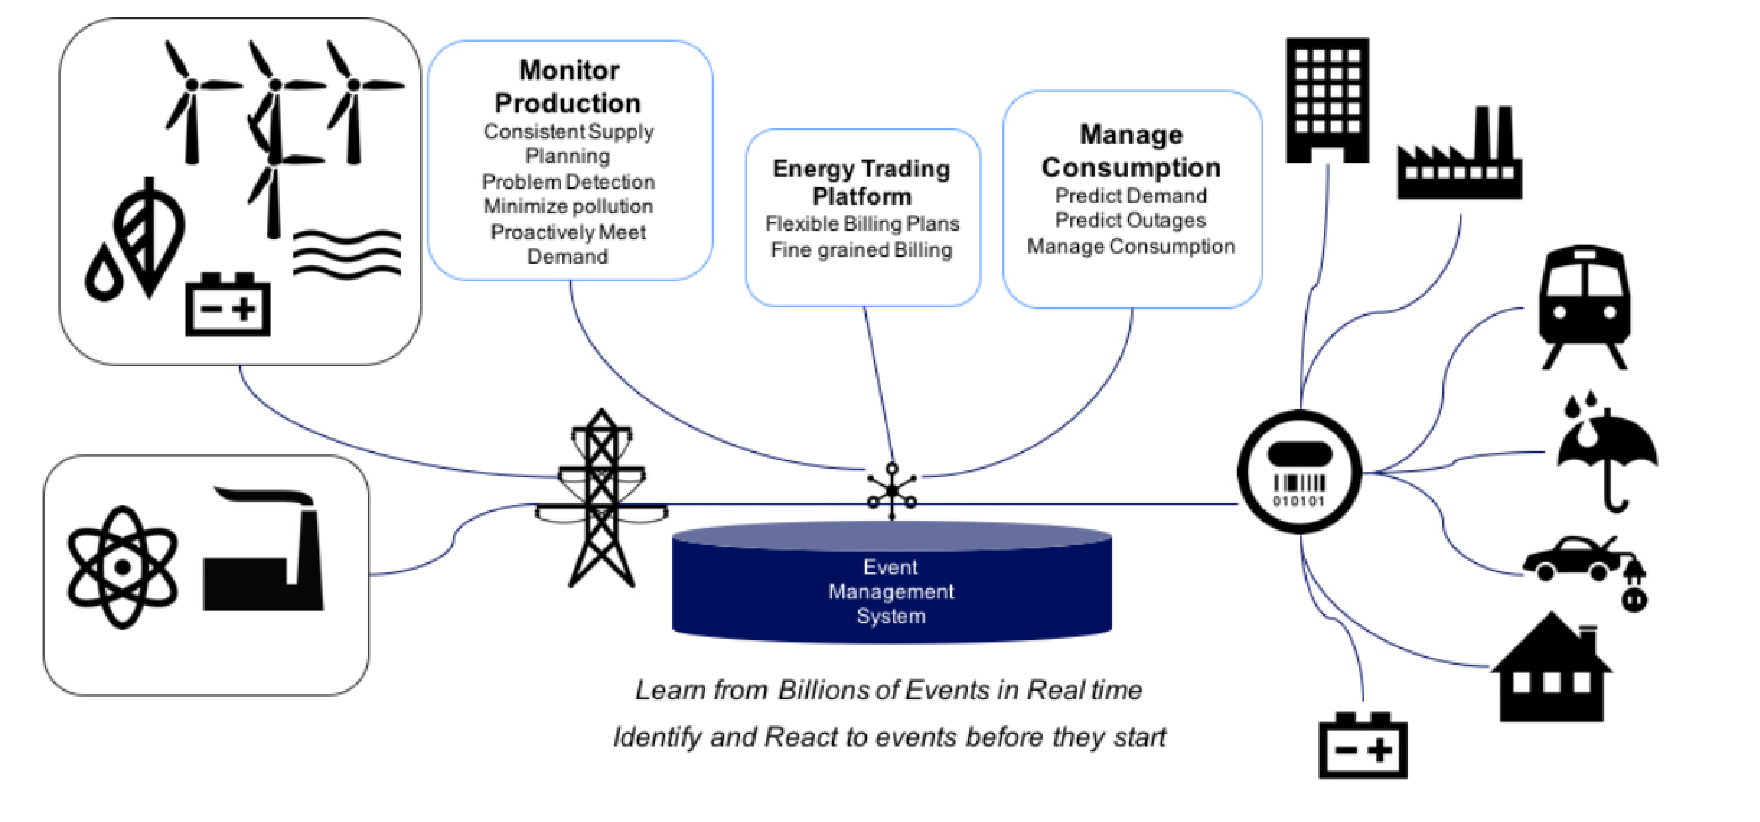
\includegraphics[width=1.0\columnwidth]{images/IBM_EventStore.pdf}
	\caption{IBM's event-driven Data Management System \cite{downey01}}
	\label{F:event}
\end{figure}
Figure \ref{F:event} shows how IBM's event-driven data management system works as an efficient analytics tool for the energy sector.\\
The advantages that these systems can provide utilities will be visible in form of cost reductions (increasing capital productivity and saving excess expenditures on operations and maintenance), increased reliability (predicting outages and accurately detecting failures of equipments) and customer satisfaction (engaging customers in the process flow by providing them with useful insights about their consumption patterns) \cite{guille02}. Some of these smart technologies have been actively deployed as well. GTM Research predicts that ``global utility company expenditure on data analytics will grow from 700 million in 2012 to 3.8 billion in 2020, with gas, electricity and water suppliers in all regions of the world increasing their investment'' \cite{callahan03}.
   

\section{The Rise of Smart Technologies}
Big Data warehouses and analytic technologies have been making waves in the energy and utilities sector for some time now. One example is of Microsoft, where 30,000 existing sensors were organized into a single energy-efficient system, at the company's Redmond, Washington, headquarters \cite{wharton04}. The network is used to avail billions of data points on energy usage in areas such as heating, cooling and lighting. Analysis of this data lead to, in one case, a garage exhaust fan, that had been running for a year and costing Microsoft 66,000 USD. Through this system, the company saves close to a ``60 million USD capital investment in energy-efficient technologies'' \cite{wharton04}. On a larger scale, there is huge amount of data available, being generated from oil wells, electricity and other utility grids, and generation stations. Using big data technologies coupled with the Internet of Things (IoT) i.e. smart sensors, all of this information can be gathered, structured and analyzed to provide valuable insights on utility management.

\subsection{Smart Meters and Grids}
A {\em Smart Meter} differs from a regular meter in its additional abilities of not only measuring the energy consumption for the customer, but also processing it and providing real-time feedback regarding it. Some of the features of a smart meter are as follows:  real-time registration of energy usage, possibility to get meter information locally and remotely, remote access of the meter for adjustment of throughput, interconnection among various devices on the premise, ability to read other commodity meters in the vicinity \cite{leonardo05}.
\begin{figure}
	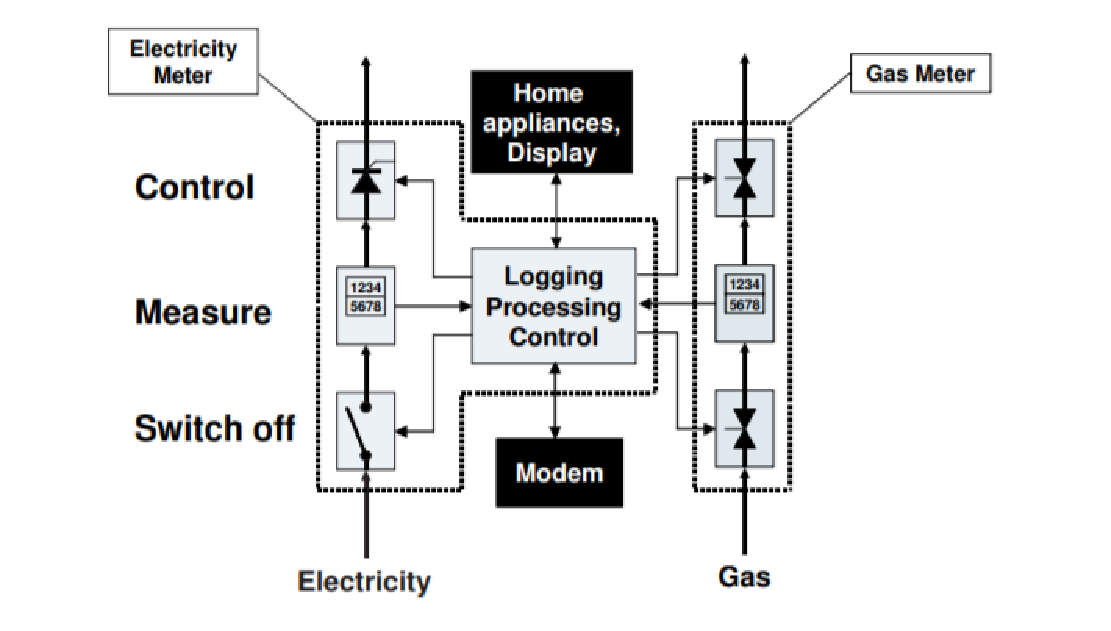
\includegraphics[width=1.0\columnwidth]{images/smart_meter.pdf}
	\caption{Typical Smart Meter Structure \cite{leonardo05}}
	\label{F:smart}
\end{figure}
Figure \ref{F:smart} shows a typical smart meter structure.\\
The {\em smartness} of a smart meter lies in its communication system. The meter can communicate using a Power Line Carrier, a wireless modem (GSM) or an existing internet connection. An interface can be used to connect this meter to appliances and a home display, using which it can show the energy data and costs to the consumer \cite{leonardo05}.\\
Though generally used for measuring energy consumption, smart meters can also be employed for other utilities such as gas and water. Smart water meters are not as common, but if implemented properly, can help detect issues such as leaks on the premises, in the main line, and wastage of water, much more promptly than with traditional technologies \cite{smartmeter09}. Smart metering technologies, in general, can prove to be an essential addition to demand response as well as predictive management techniques.\\
A {\em Smart Grid} network is an advanced form of a traditional power grid (the concept is generally applied in the electricity sector). It provides a two-way exchange of electricity and information to create a widely distributed energy-delivery system, which is reliable, resilient and sustainable \cite{fang06}. Technologies such as smart meters act as components of a smart grid framework, which acts as an intelligent system that monitors generation, transmissions and consumption in the complete electric grid and performs dynamic energy management. For example, in case of a transformer failure, the smart grid would detect it and modify the power flow such that it recovers the power delivery service \cite{fang06}. Apart from this, smart grids can also be used in shaping energy demand profiles. The three major components in a smart grid system are: smart infrastructure, smart management and smart protection. The smart infrastructure helps in advanced energy flow, monitoring and communication. The smart management system provides control services. The smart protection system ensures reliability, safety and security of the network \cite{fang06}.
\begin{figure}
	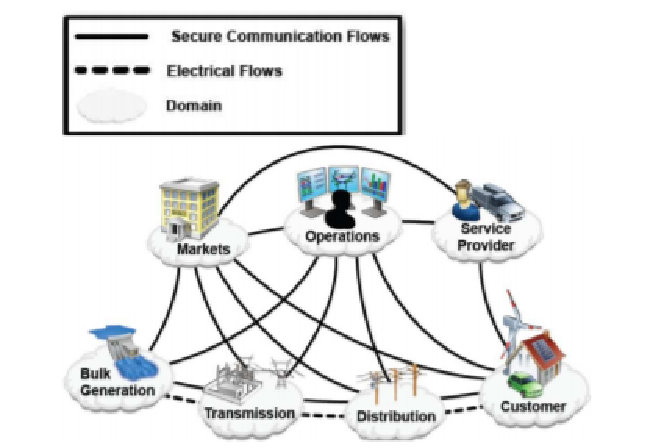
\includegraphics[width=1.0\columnwidth]{images/smart_grid.pdf}
	\caption{Conceptual model for a Smart Grid \cite{fang06}}
	\label{F:grid}
\end{figure}
Figure \ref{F:grid} shows the NIST conceptual model for a Smart Grid.\\
Thus, we see that the volume of data obtained from smart meters in smart grid networks, along with other components, can be used for a variety of intentions. For example, Diamantoulakis, Kapinas and Karagiannidis have used smart grid information for the purpose of load synchronization. Cloud computing technologies have been used to manage the big data obtained from a smart grid (using distributed data management and parallelization). Next, dimensionality reduction has been applied to keep only the useful predictors and data mining techniques like Artificial Neural Networks or Clustering have been used to model customer load curves. This has been followed by short-term load forecasting techniques (using regression, time-series or state-space models) to provide values for price and demand forecasts \cite{george07}.
\begin{figure}
	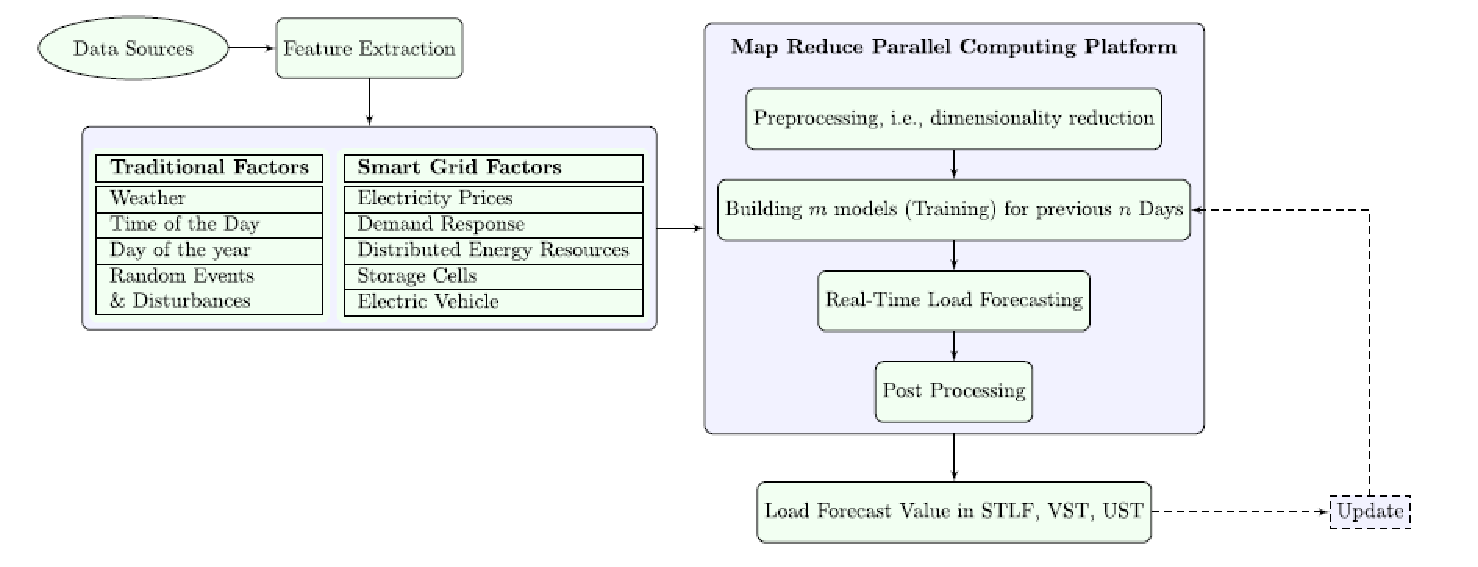
\includegraphics[width=1.0\columnwidth]{images/sg_forecast.pdf}
	\caption{Smart Grid Forecast Model \cite{george07}}
	\label{F:forecast}
\end{figure}
Figure \ref{F:forecast} shows a rough structure of the Smart Grid forecast model.

\subsection{Energy Disaggregation}
{\em Energy Disaggregation} is a novel idea born out of the possibilities offered by the smart metering technologies discussed above. It involves the breakdown of the main electric signal into consumption by each individual appliance in a unit. Also referred to as NILM (Non-Intrusive Load Monitoring), this technology can help create itemized energy bills for consumers and help them monitor their consumption in a much more specific format. This in turn helps in efficient management of the power grid as well, as the user can detect if any device is faulty or consuming more than the normal amount of energy \cite{wan08}. The data generated by smart meters can be used for this process. The main electric signal can then be broken down into signals from individual appliances by identifying their signatures. This data obtained on an individual as well as aggregate level can be analyzed using data mining techniques such as deep learning (neural networks), Combinatorial Optimization or Factorial Hidden Markov Models (FHMM) to detect patterns useful for prediction purposes \cite{wan08}.

\subsection{Electric Vehicles}
The advent of {\em Electric vehicles} has largely reduced the strain on non-renewable fossil fuels. They form an important part of the Smart Grid network discussed in the previous section. The increase in use of electric vehicles leads to beneficial reduction in carbon emissions as well. However, one major consideration in the use of electric vehicles is charging these vehicles without overloading the grid \cite{acm10}. However, data analytics can help us here by designing scheduling systems for charging of these vehicles. Control mechanisms need to be set up to guide the charging of these vehicles. Also, consumers need to be explained to or incentivized so that they follow these guidelines and ensure that the load on the electric grid is stabilized. The advantage of electric vehicles is the presence of large batteries which can store charge and often help in load shifting within the owner's home. This indirectly provides energy back to the grid and helps stabilize it as well. Optimization techniques, using the data obtained from use of these vehicles (their charging-discharging cycles and energy demands), can help in devising such load scheduling systems which prove to be beneficial units of the Smart Grid system \cite{acm10}. 


\section{Growth Areas in the Energy Industry}
The advancement of technology has led to a cultural shift in the energy industry as well. Not only are technologies changing, but also the mindsets and therefore business strategies of companies in the energy sector \cite{util11}. Some of the major areas in the industry touched by the advent of big data technologies are operations, asset management, demand-side management and customer satisfaction. Apart from these areas, the concept of sustainability is one of utmost importance. Efficient usage of renewable resources is another major benefit provided by data analytics to the energy industry.

\subsection{Asset Management and Operational Efficiency}
Managing its assets and ensuring smooth-running operations are two of the most vital, interdependent tasks for the energy industry. The assets involved in running day-to-day operations are typically quite expensive and result in service interruptions and losses if damaged. Therefore, using prediction and optimization techniques to detect and prevent possible issues in an oil well or power grid or gas pipes is extremely essential, from an asset management point of view as well as to ensure operational efficiency \cite{info12}. For example, use of complex algorithms on big data platforms like Hadoop for seismic data analysis can potentially help identify optimal drilling locations and reduce risks in the process \cite{acc15}. The increase in data being obtained from a variety of sources and the availability of useful machine learning algorithms to make sense of them has opened up opportunities to monitor and detect possible scope of anomalies or leaks and prevent them beforehand. This has also helped in efficient personnel management as it reduces unscheduled visits due to early warnings \cite{schneider13}. Maintenance staff can be better equipped to deal with equipment damages, loads can be shifted to stabilize strained networks and possible outages can be prevented. Predictive maintenance, rather than reactive maintenance, is the need of the hour. An example is Schneider Electric's Avantis PRiSM, a predictive analytics tool, which used prediction based on models built on the asset's operational history during its various phases \cite{schneider13}. In one case, a steam model turbine, which was having sporadic issues over the course of a year was fixed by the maintenance crew by taking corrective measures related to bearing vibrations. However, the issues did not end and the historical data from the turbine was sent to PRiSM for resolution, where it was discovered that thermal expansion issues were the main cause and bearing vibrations just the symptom. Had this predictive maintenance technique been used earlier, initial maintenance would have prevented the machine's issues from becoming chronic and saved millions of dollars on maintenance costs \cite{schneider13}.\\
Another big data analytics methodology has been discussed by Chen, Dokic, Stokes, Goldberg and Kezunovic, on outage prediction \cite{chen14}. Since weather phenomena are one of the top reasons for outages, the use of a Geographic Information System (GIS) to predict potential outages seems to show great promise. Weather and wind data, vegetation data and electric network data points are consolidated to create a database of all possible influences. This dataset is used along with predictive technologies to create a framework employed to predict risks and plan accordingly \cite{chen14}.\\
The discussed methodologies provide strong evidence as to how the data generated by the energy sector from its own assets (along with other external factors) can be leveraged to increase operational efficiency. Data from social networks and web browsing data are other potential sources for big data analytics which can be used as complements to existing data sources for inducing useful insights.

\subsection{Demand-Side Management and Customer Satisfaction}
{\em Demand-Side Management} or {\em Demand-Response Management} is a new approach to load management in the power sector. Generally, supply is adjusted in order to meet demands of the consumers. Demand-side management, however, suggests methods to adjust the demands in order to maintain a balance with the available supply \cite{acm10}. The most common ways used to implement this are offering financial incentives to reduce demands during peak times or automatically controlling device consumption. The emergence of smart meters and smart grids though, has made this process easier by introducing a two-way network and allowing demand-side management to be applied on the overall electric grid. The use of demand-side management can prove to be useful to the user (in reducing electricity costs) as well as to the supplier (by gaining sufficient time to synchronize the supply and demand, especially if using renewable technologies intermittently) \cite{acm10}. In a smart grid network, this can be implemented by designing an intelligent system that is able to {\em read} the grid and provide appropriate responses to changes in load dynamics. Such a system would be able to predict supply and demand trends for the grid and adjust accordingly. Also, the consumers should be willing to allow an intelligent system to manage their devices, by automatically shifting loads when needed, while clearly communicating with the consumer and asking permissions when required. To develop such a system, advanced big data analytic techniques and simulations are required which can model the grid and all the internal and external factors which affect it \cite{acm10}. Smart technologies like energy disaggregation can also help by providing the customers with an estimate of their consumption and encouraging them to take preventive measures to prevent overloading on the supplier's end, while reducing their own electricity prices. Factors like the introduction of electric vehicles can also help tremendously in this supply-demand balance strategy (through discharging to satisfy demands and reducing pressure on the grid). The coming together of all these heterogeneous agents (traditional electricity sources, electric vehicles, renewable sources) to maximize energy in the system results in a sort of distributed network often referred to as a {\em Virtual Power Plant} \cite{acm10}. The concept of a Virtual Power Plant is essential to demand-side management in its efficiency and ability to increase energy supply while minimizing costs.\\
Such demand-side management techniques involve high-scale analytics and cloud-computing technologies to deal with the vastness of network information being utilized. Computationally effective algorithms and optimization techniques are crucial to achieve the level of accuracy required. The results however, are invaluable not only to the energy sector but also to the customers through encouragement and implementation of highly efficient energy networks.

\subsection{Renewability and Sustainability}
The dependence on conventional fuels and sources of energy has increased over time. This has led to an increase in the resultant pollution as well as greater strain on these resources. Renewable energy sources provide alternative and cleaner energy options, thus improving sustainability. However, the issue that renewable energy faces is its intermittent usage. It is still developing as a potential replacement to conventional fuels. Therein lies the question of predicting  energy production from these sources. The data generated here is voluminous and varied, therefore making Big Data technologies the best option for analysis purposes. An example is a Vi-POC (Virtual Power Operating Center) designed to provide real-time forecasts of renewable energy generation \cite{mich16}. The system collects data from various power plants (wind, photovoltaic, biomass or geothermal)  along with weather data to predict the generation of energy on an aggregate and individual level. It takes care of the correlation between weather phenomena and internal factors related to the energy production system and employs a semi-supervised adaptive model for forecasting. Mondrian is used for online analytic services, Hive on Hadoop MapReduce is used as a query executor and HBase is used for data storage \cite{mich16}. The result is an efficient analytics system that provides useful intuition regarding renewable energy production. Deployment and utilization of such technologies can lead to a sustainable blend of  renewable and conventional energy sources, thus leading to an energy-efficient framework.

\section{Water Management}
Water is a resource imperative to our survival and therefore, one of the most important utility industries. Just as big data analytics has permeated the realm of energy industries, water too is an important customer. The water utility sector has always been quite fragmented, thus the arrival of big data analytics in this field is relatively new. However, there is tremendous scope for improvement and advancement in this sector as well. The concept of smart meters and grids as applied to energy can be used for water resource networks as well. In fact, we do have a lot of data available in the water industry. ``Water utilities see data from supervisory control and data acquisition (SCADA) systems, including flow statistics, online monitoring, dissolved oxygen (DO) measurements, and air flows, as well as data from laboratory information management systems (LIMS) and computerized maintenance management systems (CMMS), to name several examples'' \cite{andy17}. Significant use of this data for analytics has also begun. An excellent example can be made of Black and Veatch, an engineering company, which has developed operations optimization tools for the wastewater treatment facility at the city of Lawrence, Kansas. These will be extended further to the water treatment facility as well. The beneficial effects of consolidating all operations data in a single huge database have started becoming evident, especially for visualization purposes \cite{andy17}. Another shining example is of Fathom, a startup based mainly in the water utility data management area \cite{barb18}. The CEO of Fathom, Trevor Hill, has led the campaign to revolutionize the water utility sector by setting up a cloud-based platform to offer software-as-a-service to water utilities. Fathom provides meter-reading services on the cloud, automated billing and customer services comprising of leak and meter failure detection. Trevor Hill describes his system as a ``smart grid for water utilities'' \cite{barb18}. The rise of smart technologies is gradually, but definitely, reforming the water management sector along with other utilities.

\section{Case Studies}
Various companies in the energy and utilities sector have used big data analytics to improve their operations and customer management strategies. Each success story reveals how much big data has come along in revamping the entire industry. CenterPoint, a Houston based electric and natural gas utility, has used big data in saving itself a considerable amount of manual labor as well as costs. Physical inspections used to cost the company 88,000 meters every day (75 USD each). This changed with the deployment of smart meters which covered 221 million readings each day and with no traveling costs at all \cite{wharton04}. Oncor Electric Delivery Company LLC, the biggest electricity distribution-transmission company in Texas, collaborated with IBM and installed smart meters for its customers, thus creating an efficient and interactive energy grid and saving its consumers 25 percent and more in electricity bills. Additionally it improved its crisis-response time by almost 40 percent \cite{oncor19}. Vestas, one of the largest wind energy companies in the world, worked with IBM to implement a system that helped in locating optimal turbine placement sites and forecasting wind patterns and energy production. This system produced a 97 percent faster prediction and response time and resulted in 40 percent decrease in energy utilization while increasing computational capacity \cite{vestas21}. Podo, a Spanish utilities company, worked with Cloudera to design a prediction system for consumer energy consumption patterns. This model helped development of micro-targeted campaigns and reduced electricity bills for customers and companies up to 30 percent \cite{cloud20}. The {\em big data leap} for all these companies translated into profits and a colossal increase in operational efficiencies.

\section{Conclusions}
Implementation of big data technologies is not without its obstacles. Silos mentality and fragmented systems, along with the difficulties in consolidation of highly skilled data scientists and big data based system resources, do pose hindrances on the way to an intelligent and efficient framework. However, we see an increasing number of success stories, people willing to put in the extra effort, to develop intelligence in their systems by breaking the fetters of ignorance. With the increase in technical innovations, it is highly unlikely that the energy and utilities sector will stay behind. The current pace of big data analytics in the industry can assure us that {\em smart systems} are here to stay. 


\bibliographystyle{ACM-Reference-Format}
\bibliography{report}
